Ud fra applikationsmodellens klasse diagram (Figur \ref{fig:CSS_hovedenhed_Class}) er udledt et statisk klasse diagram, se figur \ref{fig:CSS_hovedenhed_Class_Static}.
\begin{figure}[!htb] \centering
     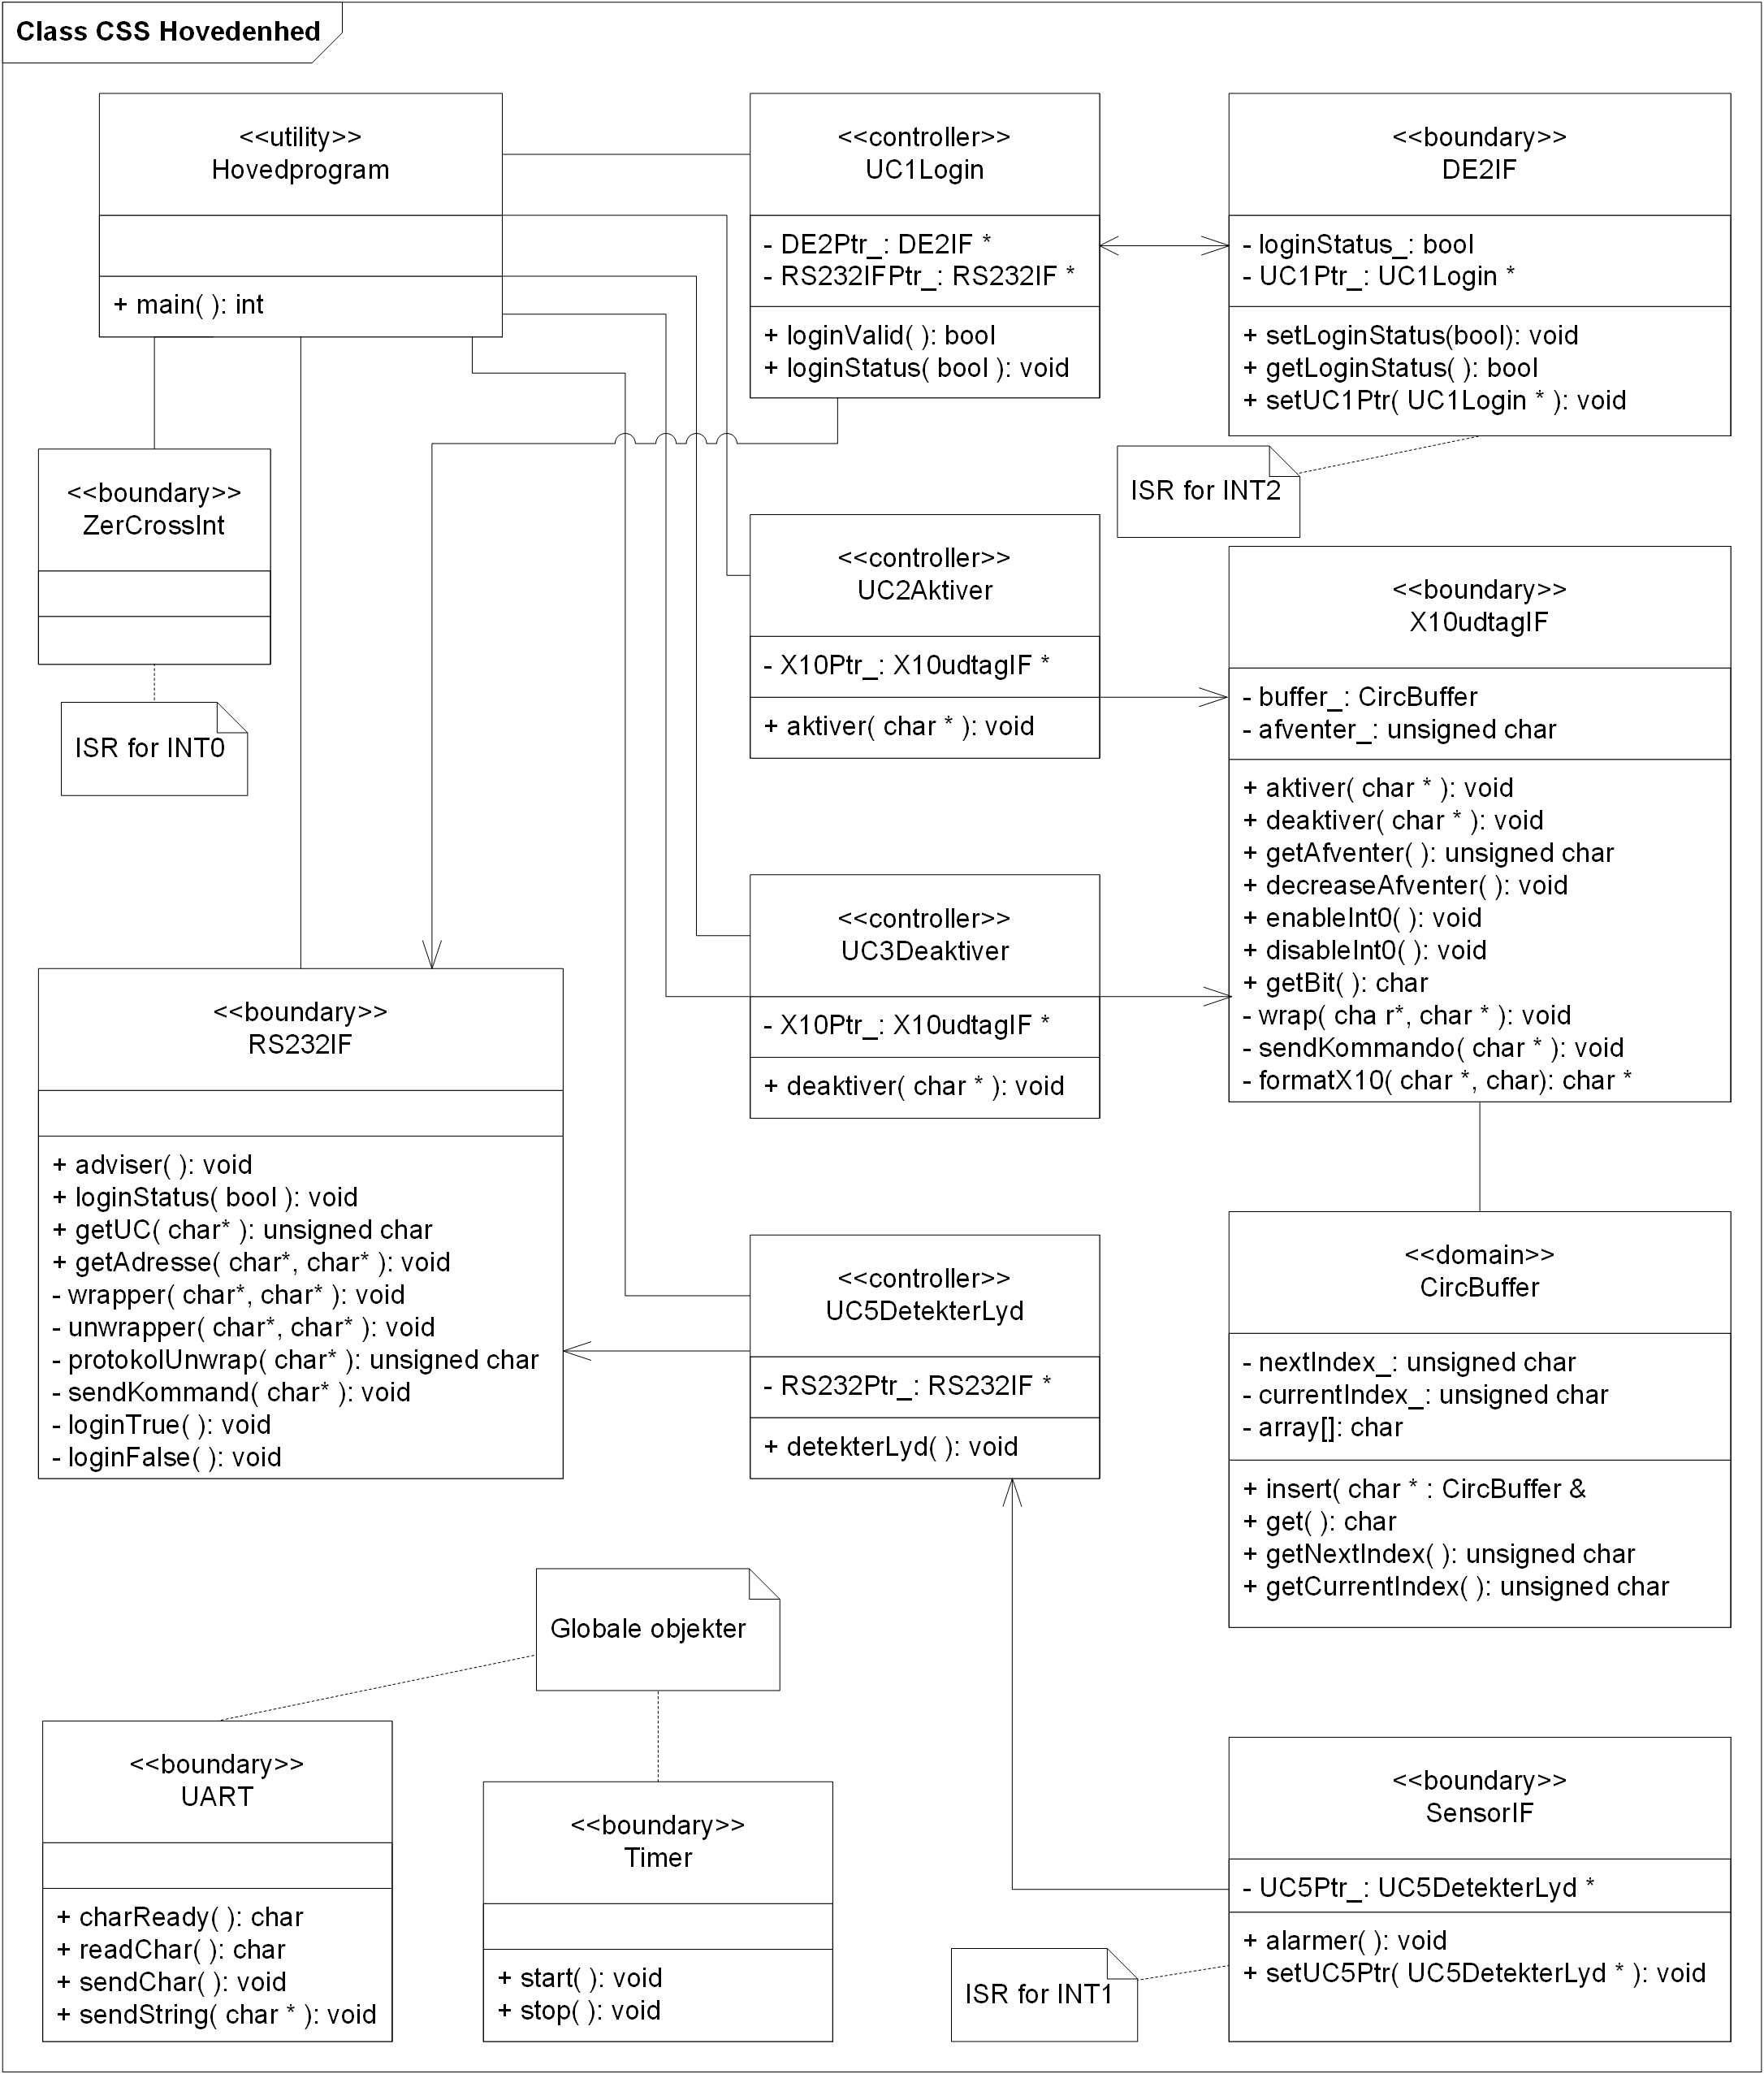
\includegraphics[width=\textwidth]{billeder/uml/CSS_hovedenhed_Class_Static}
     \caption{Statisk klassediagram for CSS hovedenhed}
     \label{fig:CSS_hovedenhed_Class_Static}
\end{figure}

Her følger klassebeskrivelser for alle klasser til CSS hovedenheden. \\

%
% RS232IF
%
{\centering
\textbf{RS232IF}\par
}
\textbf{Ansvar:} At varetage kommunikation mellem CSS hovedenhed og PC over RS232 protokollen. \\
\textbf{Attributer:}
\begin{itemize}
	\item \textbf{UC1Login * UC1Ptr\_} \\
	Pointer til associeret UC1 objekt
	\item \textbf{UC2Aktiver * UC2Ptr\_} \\
	Pointer til associeret UC2 objekt
	\item \textbf{UC3Deaktiver * UC3Ptr\_} \\
	Pointer til associeret UC3 objekt
\end{itemize}
\textbf{Metoder:} \\
void adviser(); \\
\textbf{Parametre:} Ingen \\
\textbf{Returværdi:} Ingen \\
\textbf{Beskrivelse:} Sender kommando "SB<cr>" over RS232 \\

%
% UC1Login
%
{\centering
\textbf{UC1Login}\par
}
\textbf{Ansvar:} At varetage UC1 Login forløbet. \\
\textbf{Attributer:}
\begin{itemize}
	\item \textbf{DE2IF * DE2Ptr\_} \\
	Pointer til associeret DE2 objekt
\end{itemize}
\textbf{Metoder:} \\
bool loginValid(); \\
\textbf{Parametre:} Ingen \\
\textbf{Returværdi:} Ingen \\
\textbf{Beskrivelse:} Kalder getLoginStatus() metoden i DE2IF og returnerer værdien her fra \\

%
% UC2Aktiver
%
{\centering
\textbf{UC2Aktiver}\par
}
\textbf{Ansvar:} At varetage UC2 Aktiver forløbet. \\
\textbf{Attributer:}
\begin{itemize}
	\item \textbf{X10udtagIF * X10Ptr\_} \\
	Pointer til associeret X10udtag objekt
\end{itemize}
\textbf{Metoder:} \\
void aktiver(int adresse); \\
\textbf{Parametre:} Adresse på enhed \\
\textbf{Returværdi:} Ingen \\
\textbf{Beskrivelse:} Kalder aktiver() metoden i X10udtagIF med den modtagede adresse \\

%
% UC3Deaktiver
%
{\centering
\textbf{UC3Deaktiver}\par
}
\textbf{Ansvar:} At varetage UC3 Deaktiver forløbet. \\
\textbf{Attributer:}
\begin{itemize}
	\item \textbf{X10udtagIF * X10Ptr\_} \\
	Pointer til associeret X10udtag objekt
\end{itemize}
\textbf{Metoder:} \\
void deaktiver(int adresse); \\
\textbf{Parametre:} Adresse på enhed \\
\textbf{Returværdi:} Ingen \\
\textbf{Beskrivelse:} Kalder deaktiver() metoden i X10udtagIF med den modtagede adresse \\

%
% UC5DetekterLyd
%
{\centering
\textbf{UC5DetekterLyd}\par
}
\textbf{Ansvar:} At varetage UC5 Detekter Lyd. \\
\textbf{Attributer:}
\begin{itemize}
	\item \textbf{RS232IF * RS232Ptr\_} \\
	Pointer til associeret X10udtag objekt
\end{itemize}
\textbf{Metoder:} \\
void detekterLyd(); \\
\textbf{Parametre:} Ingen \\
\textbf{Returværdi:} Ingen \\
\textbf{Beskrivelse:} Kalder adviser() metoden i RS232IF \\

%
% DE2IF
%
{\centering
\textbf{DE2IF}\par
}
\textbf{Ansvar:} At holde styr på aktuel loginstatus på DE2 boardet. \\
\textbf{Attributer:}
\begin{itemize}
	\item \textbf{bool loginStatus\_} \\
	1: Login bekræftet på DE2 board \\
	0: Login ikke bekræftet på DE2 board
\end{itemize}

\textbf{Metoder:} \\
void setLoginStatus(bool status); \\
\textbf{Parametre:} status: 1 hvis bekræftet og 0 hvis ikke bekræftet på DE2 board \\
\textbf{Returværdi:} Ingen \\
\textbf{Beskrivelse:} Sætter attribut loginStatus\_ til aktuel status på DE2 board \\

bool getLoginStatus(); \\
\textbf{Parametre:} Ingen \\
\textbf{Returværdi:} status: 1 hvis bekræftet og 0 hvis ikke bekræftet på DE2 board \\
\textbf{Beskrivelse:} Returnerer aktuel login status \\

%
% X10udtagIF
%
{\centering
\textbf{X10udtagIF}\par
}
\textbf{Ansvar:} At varetage kommunikation mellem CSS hovedenhed og X10 modtager over X10 protokollen. \\
\textbf{Attributer:} Ingen \\
\textbf{Metoder:} \\
void aktiver(int adresse); \\
\textbf{Parametre:} adresse: Adresse på X10 enhed som ønskes aktiveret \\
\textbf{Returværdi:} Ingen \\
\textbf{Beskrivelse:} Konverterer adressen bitvis til ASCII karrakterer (0010 -> ''0010'') og sender kommandoen "SAXXXX<cr>" (hvor XXXX er adressen over) over X10 \\

void deaktiver(int adresse); \\
\textbf{Parametre:} adresse: Adresse på X10 enhed som ønskes deaktiveret \\
\textbf{Returværdi:} Ingen \\
\textbf{Beskrivelse:} Konverterer adressen bitvis til ASCII karrakterer (0010 -> ''0010'') og sender kommandoen "SDXXXX<cr>" (hvor XXXX er adressen over) X10 \\

%
% SensorIF
%
{\centering
\textbf{SensorIF}\par
}
\textbf{Ansvar:} At holde styr på aktuel lyd detektering og give besked hvis lyd registreres. \\
\textbf{Attributer:}
\begin{itemize}
	\item \textbf{bool loginStatus\_} \\
	1: Lyd detekteret \\
	0: Ingen lyd detekteret
	\item \textbf{UC5DetekterLyd * UC5Ptr\_} \\
	Pointer til associeret UC5 objekt
\end{itemize}

\textbf{Metoder:} \\
void setLydNiveau(bool niveau); \\
\textbf{Parametre:} niveau: 1 hvis lyd detekteret ellers 0 \\
\textbf{Returværdi:} Ingen \\
\textbf{Beskrivelse:} Kalder detekterLyd() metoden, i UC5DetekterLyd, med parameter 1, hvis niveau er 1, ellers intet. \\

